\section{Architecture}
\label{sec:arch}

Four parallel processes exist being \emph{signs}, \emph{barriers}, \emph{bridge} and \emph{safety layer}. \emph{Signs} handles the control of the lights, whereas \emph{barriers} handles the barriers and \emph{Bridge} the locks and the deck. \emph{Safety layer} makes sure that the input from the bridge operator can only be executed if the conditions are so safe, so no accidents like the Ketelbrug will be possible. The structure of this setup can be explained as follows:
%
\begin{itemize}
	\item \emph{Safety layer} is the process that accepts all possible inputs
		that are allowed by the bridge operator. For every command, the safety
		layer knows what current states of the individual components are
		required for the execution to be safe. For checking whether these
		requirements are fulfilled, it requests the three processes
		\emph{signs}, \emph{barriers} and \emph{bridge} for a status by means
		of a \texttt{receive}-action.  When the command is considered safe,
		\emph{Safety layer} informs the processes by means of
		\texttt{s}-actions. When these are answered by \texttt{r}-actions, a
		communication (\texttt{c}) action is established and the command is
		executed.
	\item \emph{Signs} is the process that holds the sensor values for the pre and stop signs. Recall that our assumption is that the status of the process is the value detected by the majority of the sensors. When the safety layer
	requests the status of a sign, the process sends out a \texttt{send}-action in return. Together with the \texttt{receive}-action from the safety layer, a \texttt{comm}-action is formed upon which the safety layer bases its
	judgement for safety. When receiving an \texttt{s}-action from the safety layer, \emph{Signs} returns a \texttt{r}-action to confirm the execution.
	\item \emph{Barriers} is the process that holds the sensor values for the front and back barriers. Recall that our assumption is that the status of the process is the value detected by the majority of the sensors. When the
	safety layer requests the status of a barrier, the process sends out a \texttt{send}-action in return. Together with the \texttt{receive}-action from the safety layer, a \texttt{comm}-action is formed upon which the safety layer
	bases its judgement for safety. When receiving an \texttt{s}-action from the safety layer, \emph{Barrier} returns a \texttt{r}-action to confirm the execution.
	\item \emph{Bridge} is the process that holds the sensor values for the locks and bridge deck. Recall that our assumption is that the status of the process is the value detected by the majority of the sensors. When the
	safety layer requests the status of a lock or deck, the process sends out a \texttt{send}-action in return. Together with the \texttt{receive}-action from the safety layer, a \texttt{comm}-action is formed upon which the safety
	layer 	bases its judgement for safety. When receiving an \texttt{s}-action from the safety layer, \emph{Bridge} returns a \texttt{r}-action to confirm the execution.
\end{itemize}
%
Figure~\ref{fig:arch} shows a diagram of the communication flow between these parallel processes. As you can see, also the global actions that are available to the bridge operator are included. They are pictured as italic actions from outside the system that enter the safety layer on the upper side.
%
\begin{figure}[htb]%
\centering
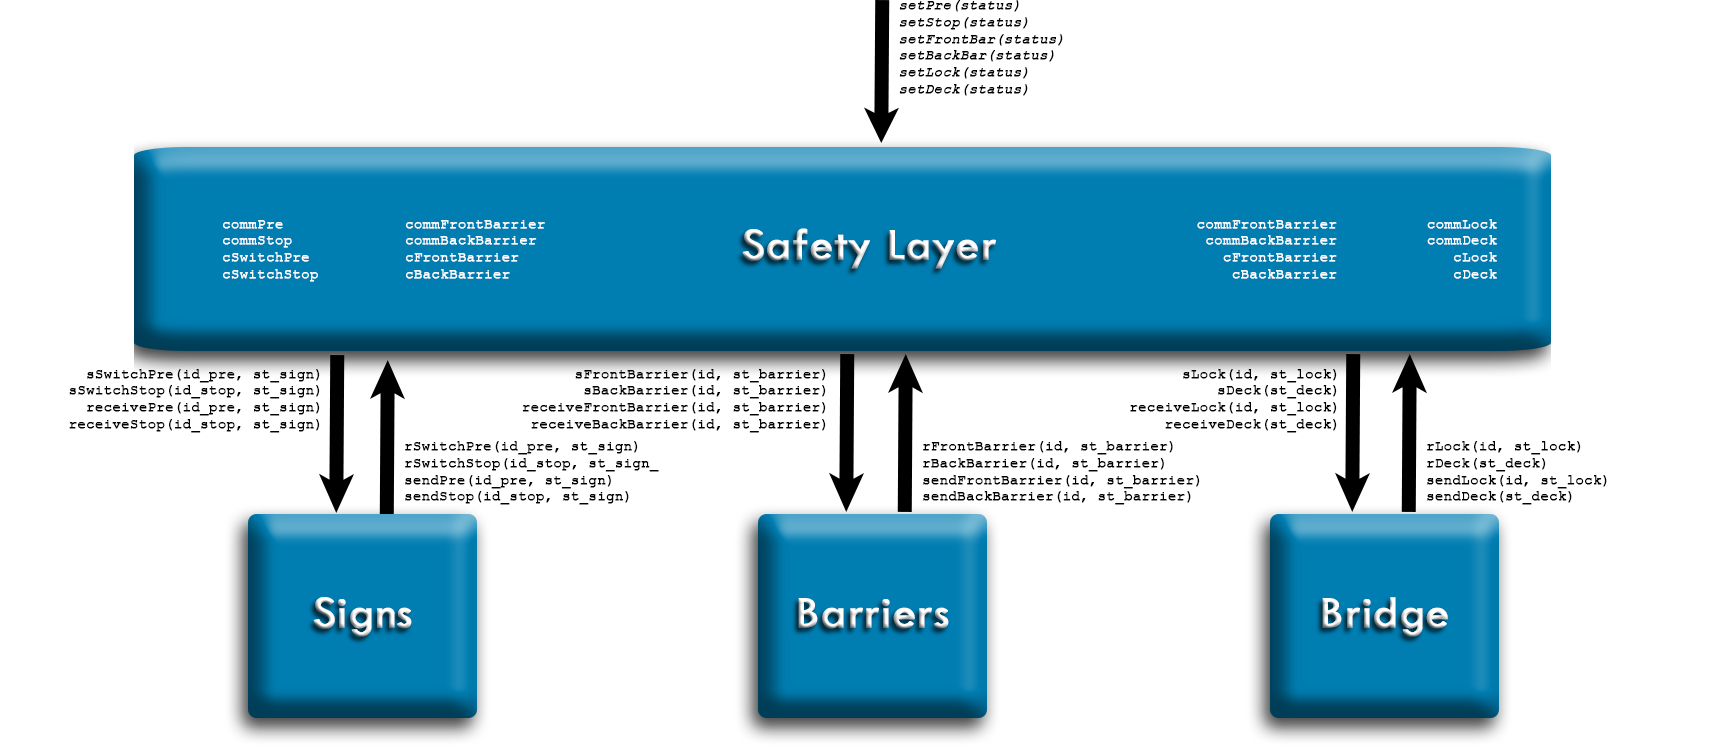
\includegraphics[width=\columnwidth, angle=90]{Images/Architecture_2}%
\caption{Communication flow between parallel processes \emph{signs}, \emph{barriers} and \emph{bridge}.}%
\label{fig:arch}%
\end{figure}
%

